\documentclass[a4paper]{article}

\usepackage[english]{babel}
\usepackage[utf8]{inputenc}
\usepackage{amsmath}
\usepackage{graphicx}
\usepackage{subfigure}

\usepackage[colorinlistoftodos]{todonotes}
% 导入包
\usepackage{hyperref}
% 格式设置
\hypersetup{hidelinks,
	colorlinks=true,
	allcolors=black,
	pdfstartview=Fit,
	breaklinks=true}
	
\title{DAT094 Lab 4:  Downloading and evaluating on the FPGA}

\author{Weihan Gao – weihanga@chalmers.se}

\date{\today}

\begin{document}
\sloppy
\maketitle


\section{Introduction}
\label{sec:introduction}
In this lab, we had two implementations of digital filters for two different times of averages and tested their hardware cost and performance. And tested the implementation with external stimuli on FPGA.

\section{The system}
The top design file MAC\_gen\_min\_full.vhdl has contains 7 components: MAC\_gen\_min\_12\_17, two convert\_data\_format, sample\_clock, SPI\_clock, SPI\_AD, and SPI\_DA with some signal lines. SPI\_AD and the following converter modules can convert the analog signal into digital signed\_data, filtered by the MAC\_gen\_min\_12\_17. After through the converter module again, the filtered signal is converted to analog data by SPI\_DA module. SPI\_clock and sample\_clock can create the clock\_enable signals.


The MAC\_gen\_min\_full module is for the average filter algorithm. It calculates the filtered data using the average from a finite number of input data sampled. The finite number is the number of TAPs, which is decided by GENERIC parameters. The SIGNAL\_WIDTH and COEFF\_WIDTH in GENERIC decide the data line width for calculation – DA\_data/AD\_data between SPI\_DA/SPI\_AD and converter, filtered\_data/signed\_data between converter and MAC\_gen\_min. Therefore, they control the hardware area (more TAPs, more area), critical set-up time constraints (more TAPs, longer time), dynamic power (because wider data lines mean more states in SPI\_FSM so that a greater number of bits to be flipped), and energy per operation.


\newpage
\newpage

\begin{figure}[h]
\centering
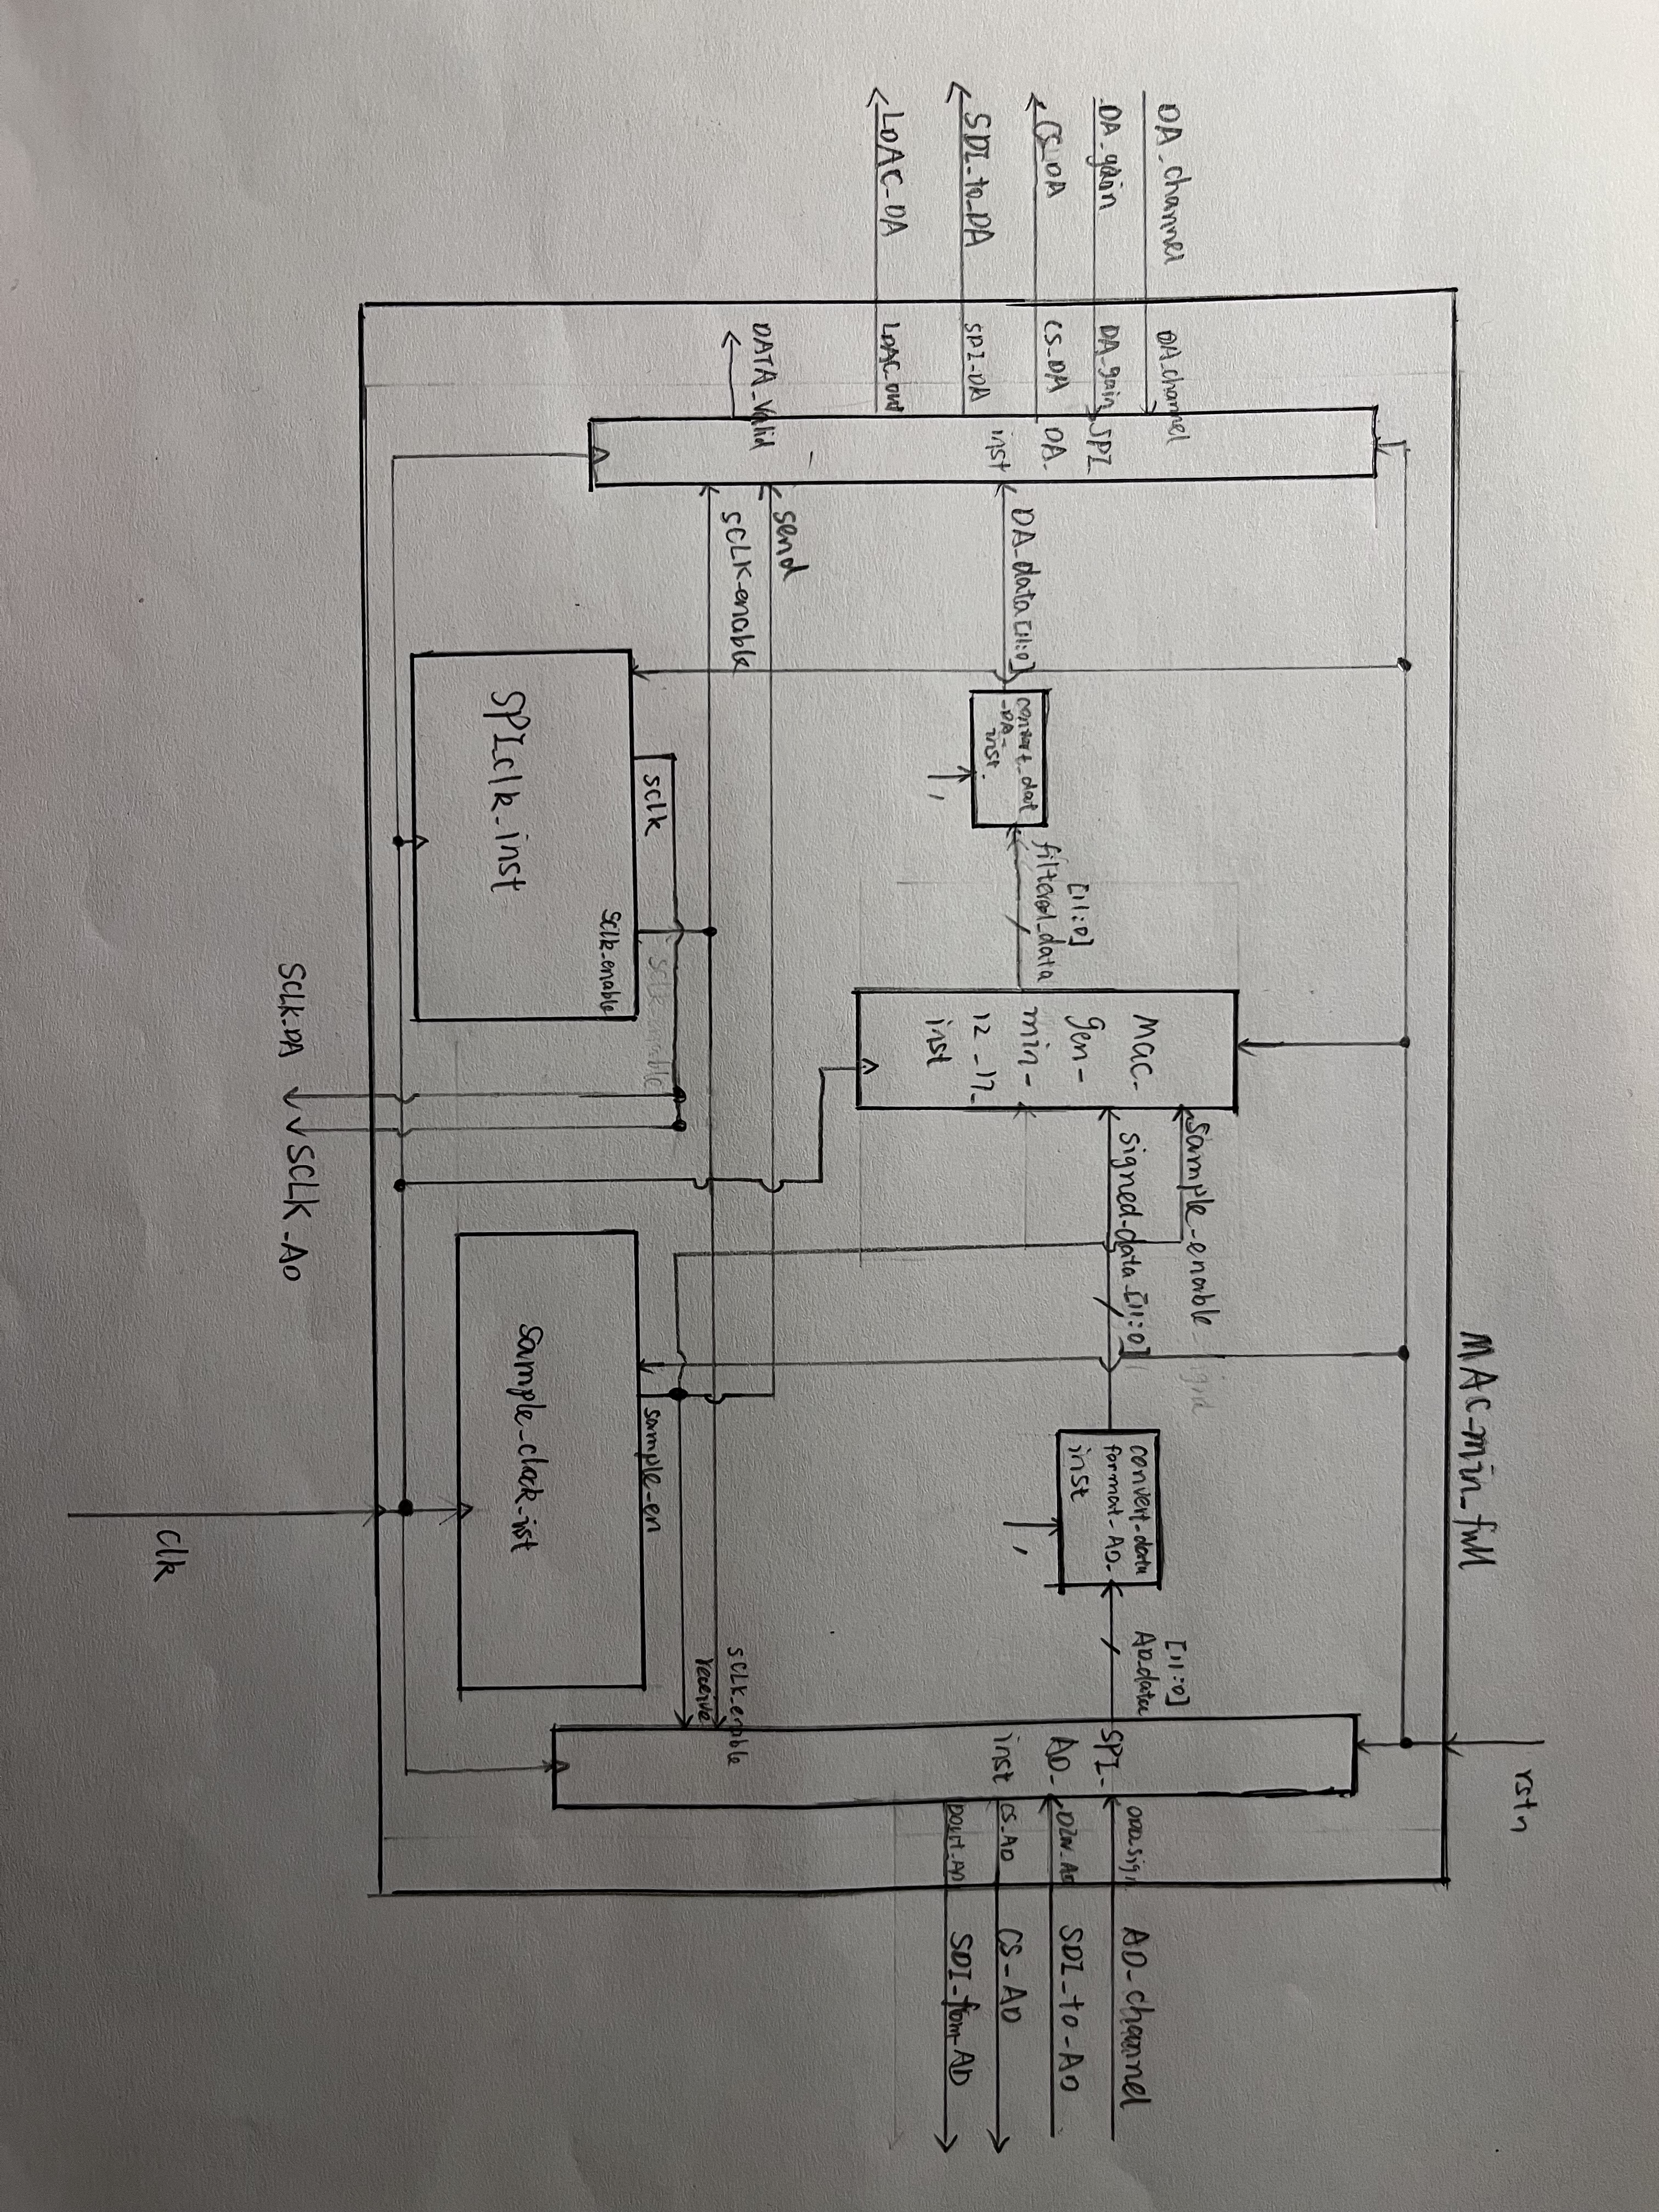
\includegraphics[width=0.9\textwidth]{1.JPG}
\caption{\label{fig:data}Block diagram.}
\end{figure}


In lab 3, we have seen that the SPI\_DA converts the parallel data into serial data by FSM. SCLK\_enable signal from the block SPI\_CLK decides how much and how long the FSM is. When we want the wordlengths of signal is 17, the necessary number of FSM is 17 (regardless of configuration and others), which means, the valid number of SCLK\_enable is 17 to change the states converting. SCLK\_en and sample\_en are generated from the frequency dividers. SPI\_CLK block, for example, has a counter counting the number of rising edge of system clk, and when it comes to the PERIOD\_constant we set, the SCLK\_en will reverse. So the period of output clock is PERIOD\_constant multiplying the system period.


The highest system clock frequency we found is about 41.7 MHz with a 0.171 ns slack. In lab3, the highest frequency is 51 MHz, higher than 41.7 MHz. It may be because of some converter combinational blocks on the critical path. The hardware utilization is also different from those in lab 3. It has 70 more LUTs and some DSPs in this design. DSP accounts for 5\% of resources near the 6\% IO. And the new serial design has same structure as the previous. The highest frequency we found is 1/9.2 = 10.9 MHz.



\begin{figure}[h]
\centering
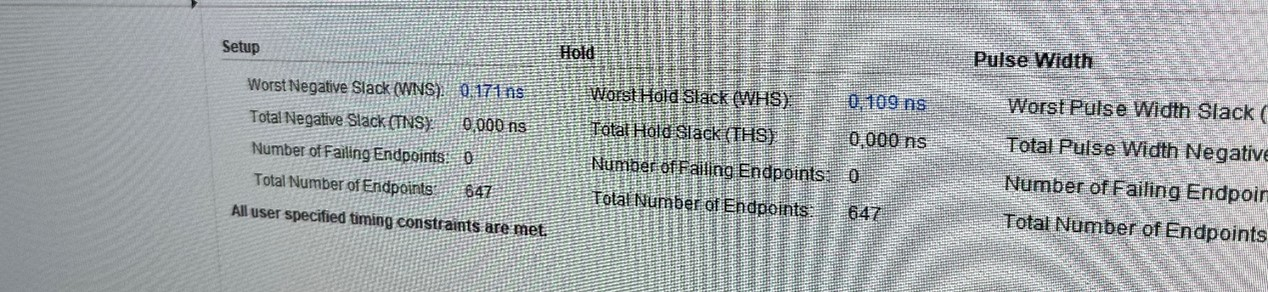
\includegraphics[width=1\textwidth]{2.jpg}
\caption{\label{fig:data}Time.}
\end{figure}

\begin{figure}[h]
\centering
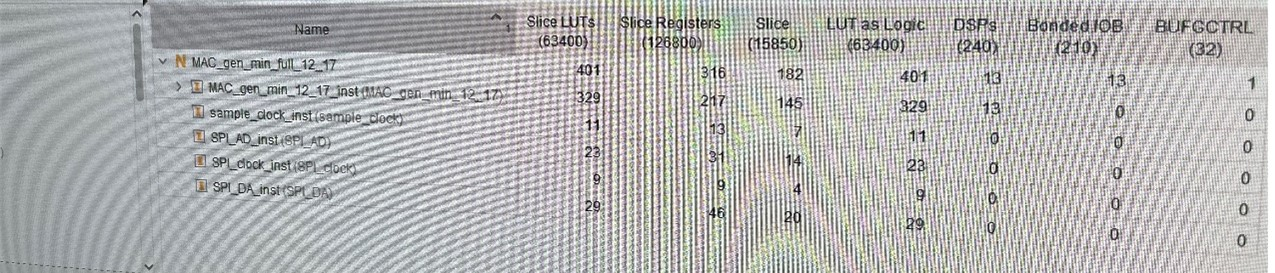
\includegraphics[width=1\textwidth]{3.jpg}
\caption{\label{fig:data}Utilization.}
\end{figure}


\begin{figure}[h]
\centering
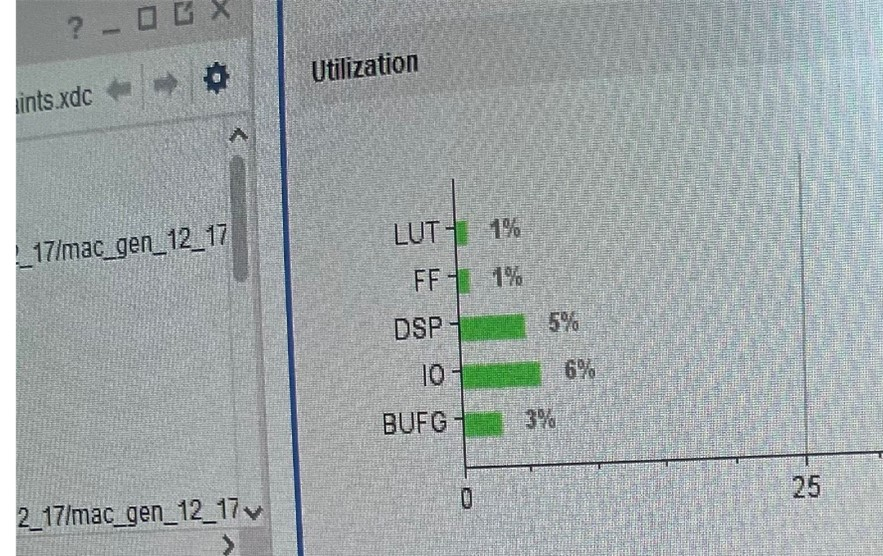
\includegraphics[width=0.8\textwidth]{4.jpg}
\caption{\label{fig:data}Utilization.}
\end{figure}

\newpage
\section{Exexute on FPGA}
We set the 1 KHz sinewave 1Vpp signal on AD input and used the oscilloscope to monitor this signal on channel 2 and DA output on channel 1. The output amplitude is related to the input signal frequency. We scanned the frequency from zero up and found when it came to 10.86 KHz, it would reduce to about $660/940=1/\sqrt{2}$. It means this design is a low-pass filter with 10.86 KHz cutoff frequency.



\begin{figure}[h]
\centering
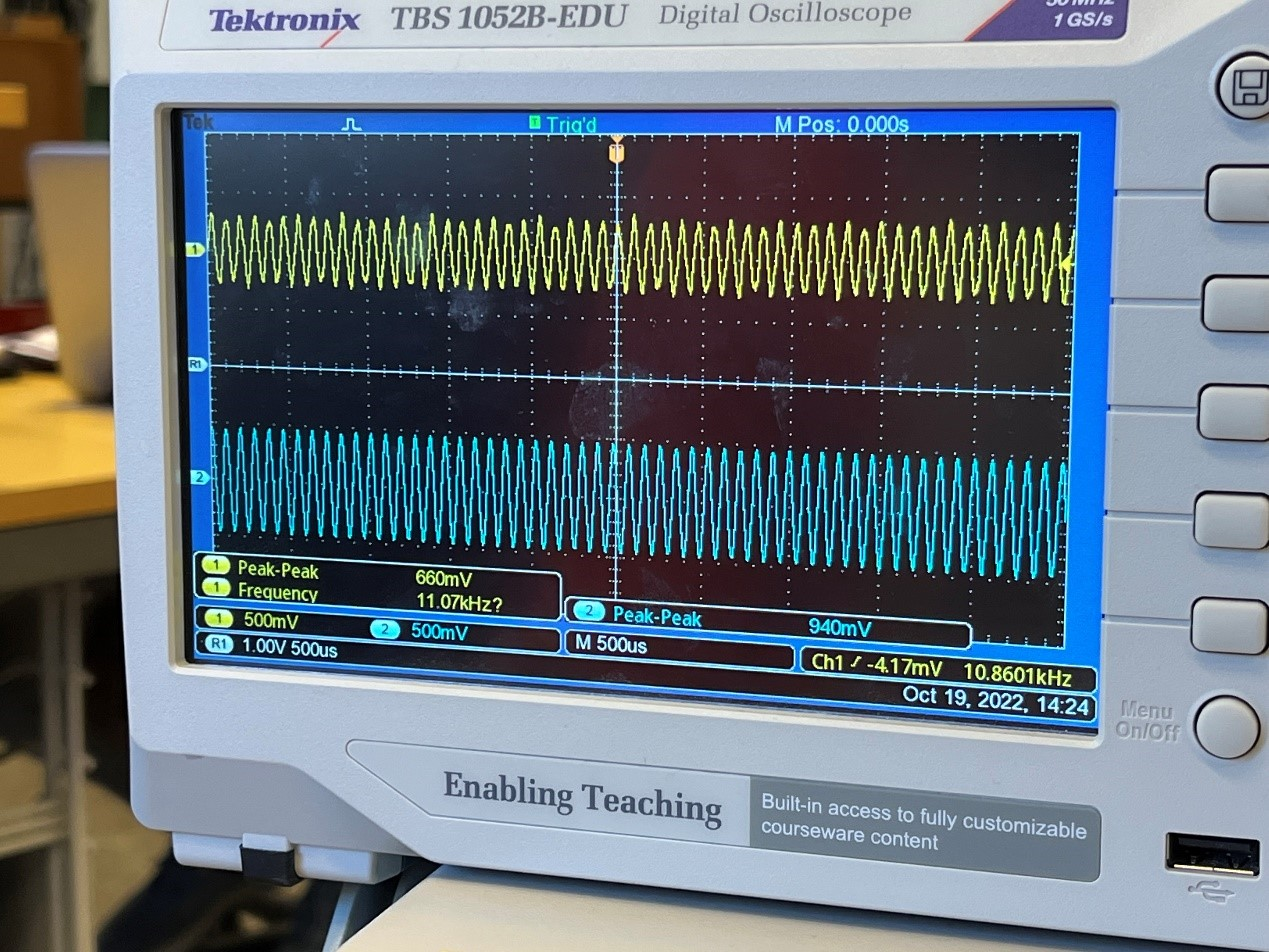
\includegraphics[width=1\textwidth]{5.jpg}
\caption{\label{fig:data}Wave of input and output.}
\end{figure}




\newpage
\section{A second parameter set}
The differences in the MAC\_gen\_min are bigger than those in the MAC\_gen\_ser. As the number of TAPs increases, the resource utilization for MAC\_gen\_min is bigger, mainly the DSP resource, increasing from 5\% to 23\%. LUT is 2780 more than the previous number. And the highest frequency is about 1/124ns = 8.1 MHz with a 0.8 ns slack.

\begin{figure}[h]
\centering
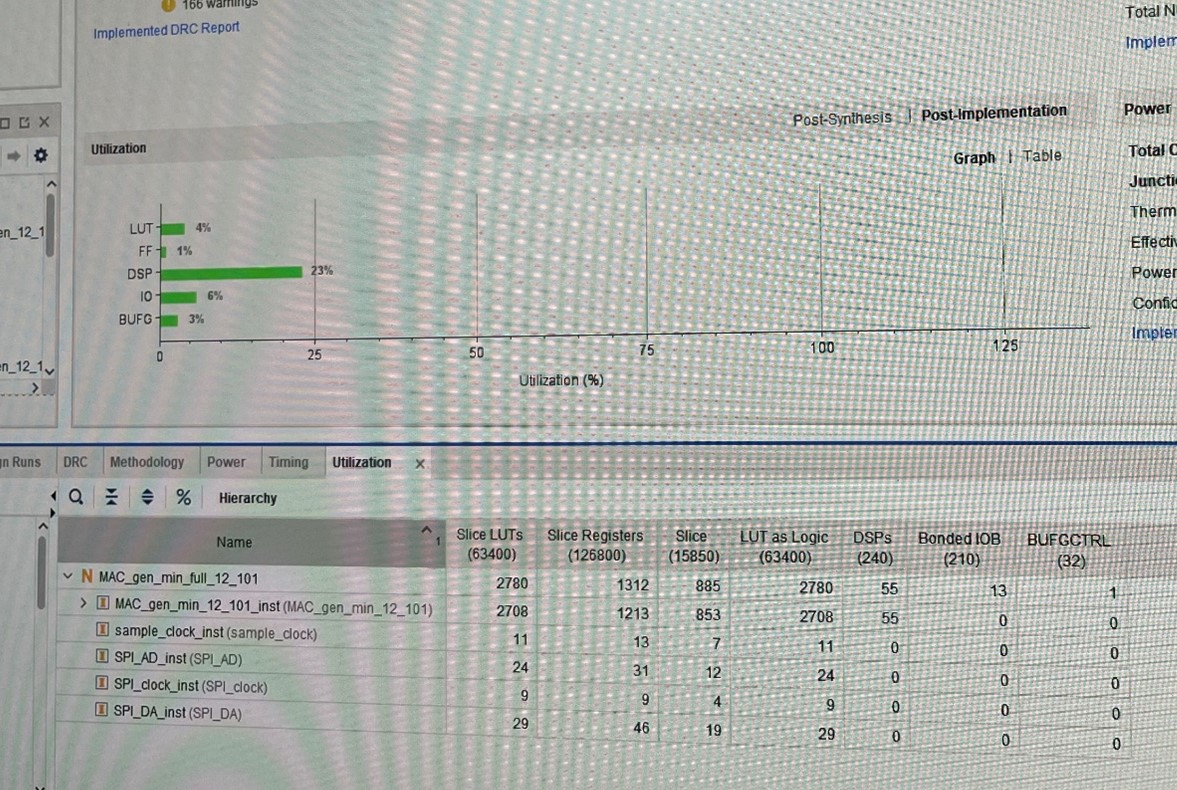
\includegraphics[width=1\textwidth]{6.jpg}
\caption{\label{fig:data}Utilization.}
\end{figure}


\begin{figure}[h]
\centering
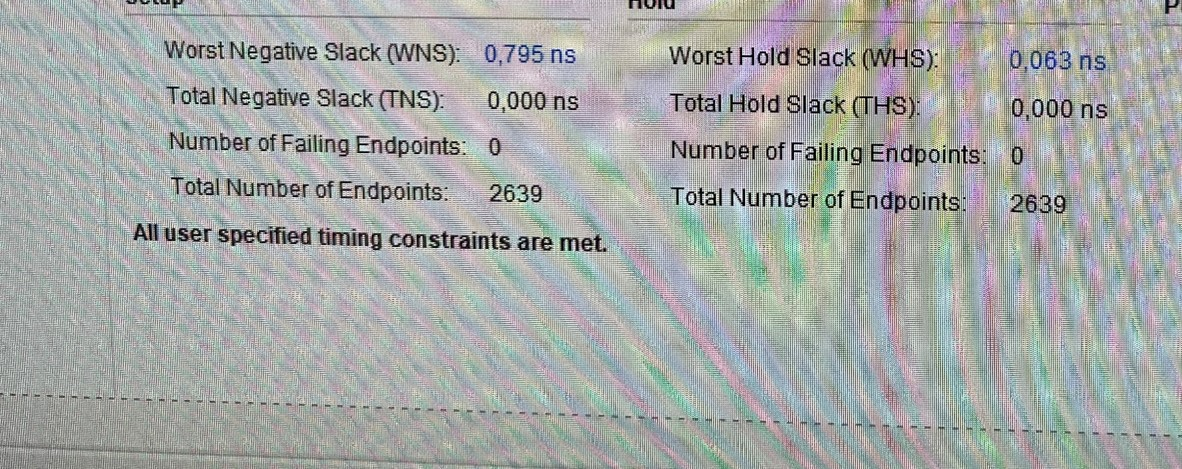
\includegraphics[width=1\textwidth]{7.jpg}
\caption{\label{fig:data}Time.}
\end{figure}



Another difference is in the frequency domain. This one is a band-pass filter rather than low-pass filter. Its cutoff frequency is 8.14 KHz and 12.84 KHz.






\newpage

\section{Summary}

Several filters have several algorithms, performances, hardware utilizations, and signal processing quality. Even if the same algorithm is, the different implementations will result in differences. If we want the smoother FIR filtered signal, we may need more TAPs, but it will change the frequency domain. So we need to make some trade-off also in the insights of signal processing.





%


%
%
%
%
%
%
%
%\begin{figure}[h]
%%\centering
%\subfigure[after Synthesis]
%{
%    \begin{minipage}[b]{1\linewidth}
%        \centering
%        \includegraphics[scale=0.7]{19.png}
%    \end{minipage}
%}
%\subfigure[after Implementation]
%{
% 	\begin{minipage}[b]{1\linewidth}
%        \centering
%        \includegraphics[scale=0.7]{20.png}
%    \end{minipage}
%}
%
%\caption{Timing in new design.}
%\end{figure}

\newpage





























\iffalse
\section{Experiment 1-2 pages}
\subsection{Fabrication}
Explain a step-by-step recipe for fabrication here. How long did you etch and why? What is an Ohmic contact?
\subsection{Experimental set-up}
Explain the experimental set-up here. Use a schematic picture (make it yourself in photoshop, paint, ...) to show how the components are connected. Briefly explain how a lock-in amplifier works.

\section{Results and interpretation 2-3 pages}
Show a graph of the longitudinal resistivity ($\rho_{xx}$) and Hall resistivity ($\rho_{xy}$) versus magnetic field, extracted from the raw data shown in figure \ref{fig:data}. You will have the link to the data in your absalon messages, if not e-mail Guen (guen@nbi.dk). Explain how you calculated these values, and refer to the theory.

\begin{figure}
\centering
\includegraphics[width=1\textwidth]{raw_data.png}
\caption{\label{fig:data}Raw (unprocessed) data. Replace this figure with the one you've made, that shows the resistivity.}
\end{figure}

\subsection{Classical regime}
Calculate the sheet electron density $n_{s}$ and electron mobility $\mu$ from the data in the low-field regime, and refer to the theory in section \ref{sec:theory}. Explain how you retrieved the values from the data (did you use a linear fit?).
Round values off to 1 or 2 significant digits: 8.1643 ~= 8.2. Also, 5e-6 is easier to read than 0.000005.

!OBS: This part is optional (only if you have time left).
Calculate the uncertainty as follows: \newline $u(f(x, y, z)) = \sqrt{(\frac{\delta f}{\delta{x}} u(x))^{2} + (\frac{\delta f}{\delta{y}} u(y))^{2} + (\frac{\delta f}{\delta{z}} u(z))^{2}}$, where $f$ is the calculated value ($n_{s}$ or $\mu$), $x, y, z$ are the variables taken from the measurement and $u(x)$ is the uncertainty in x (and so on).

\subsection{Quantum regime}
Calculate $n_{s}$ for the high-field regime.
Show a graph of the longitudinal conductivity ($\rho_{xx}$) and Hall conductivity($\rho_{xy}$) \textbf{in units of the resistance quantum} ($\frac{h}{e^{2}}$), depicting the integer filling factors for each plateau.
Show a graph of the plateau number versus its corresponding value of $1/B$. From this you can determine the slope, which you use to calculate the electron density.
Again, calculate the uncertainty for your obtained values.

\section{Discussion 1/2-1 page}
Discuss your results. Compare the two values of $n_{s}$ that you've found in the previous section. Compare your results with literature and comment on the difference. If you didn't know the value of the resistance quantum, would you be able to deduce it from your measurements? If yes/no, why?

\newpage
\section{Some LaTeX tips}
\label{sec:latex}
\subsection{How to Include Figures}

First you have to upload the image file (JPEG, PNG or PDF) from your computer to writeLaTeX using the upload link the project menu. Then use the includegraphics command to include it in your document. Use the figure environment and the caption command to add a number and a caption to your figure. See the code for Figure \ref{fig:frog} in this section for an example.

\begin{figure}
\centering
\includegraphics[width=0.3\textwidth]{frog.jpg}
\caption{\label{fig:frog}This frog was uploaded to writeLaTeX via the project menu.}
\end{figure}

\subsection{How to Make Tables}

Use the table and tabular commands for basic tables --- see Table~\ref{tab:widgets}, for example.

\begin{table}
\centering
\begin{tabular}{l|r}
Item & Quantity \\\hline
Widgets & 42 \\
Gadgets & 13
\end{tabular}
\caption{\label{tab:widgets}An example table.}
\end{table}

\subsection{How to Write Mathematics}

\LaTeX{} is great at typesetting mathematics. Let $X_1, X_2, \ldots, X_n$ be a sequence of independent and identically distributed random variables with $\text{E}[X_i] = \mu$ and $\text{Var}[X_i] = \sigma^2 < \infty$, and let

\begin{equation}
S_n = \frac{X_1 + X_2 + \cdots + X_n}{n}
      = \frac{1}{n}\sum_{i}^{n} X_i
\label{eq:sn}
\end{equation}

denote their mean. Then as $n$ approaches infinity, the random variables $\sqrt{n}(S_n - \mu)$ converge in distribution to a normal $\mathcal{N}(0, \sigma^2)$.

The equation \ref{eq:sn} is very nice.

\subsection{How to Make Sections and Subsections}

Use section and subsection commands to organize your document. \LaTeX{} handles all the formatting and numbering automatically. Use ref and label commands for cross-references.

\subsection{How to Make Lists}

You can make lists with automatic numbering \dots

\begin{enumerate}
\item Like this,
\item and like this.
\end{enumerate}
\dots or bullet points \dots
\begin{itemize}
\item Like this,
\item and like this.
\end{itemize}
\dots or with words and descriptions \dots
\begin{description}
\item[Word] Definition
\item[Concept] Explanation
\item[Idea] Text
\end{description}

We hope you find write\LaTeX\ useful, and please let us know if you have any feedback using the help menu above.

\begin{thebibliography}{9}
\bibitem{nano3}
  K. Grove-Rasmussen og Jesper Nygård,
  \emph{Kvantefænomener i Nanosystemer}.
  Niels Bohr Institute \& Nano-Science Center, Københavns Universitet

\end{thebibliography}
\fi



\end{document}